
%% bare_conf.tex
%% V1.3
%% 2007/01/11
%% by Michael Shell
%% See:
%% http://www.michaelshell.org/
%% for current contact information.
%%
%% This is a skeleton file demonstrating the use of IEEEtran.cls
%% (requires IEEEtran.cls version 1.7 or later) with an IEEE conference paper.
%%
%% Support sites:
%% http://www.michaelshell.org/tex/ieeetran/
%% http://www.ctan.org/tex-archive/macros/latex/contrib/IEEEtran/
%% and
%% http://www.ieee.org/

%%*************************************************************************
%% Legal Notice:
%% This code is offered as-is without any warranty either expressed or
%% implied; without even the implied warranty of MERCHANTABILITY or
%% FITNESS FOR A PARTICULAR PURPOSE!
%% User assumes all risk.
%% In no event shall IEEE or any contributor to this code be liable for
%% any damages or losses, including, but not limited to, incidental,
%% consequential, or any other damages, resulting from the use or misuse
%% of any information contained here.
%%
%% All comments are the opinions of their respective authors and are not
%% necessarily endorsed by the IEEE.
%%
%% This work is distributed under the LaTeX Project Public License (LPPL)
%% ( http://www.latex-project.org/ ) version 1.3, and may be freely used,
%% distributed and modified. A copy of the LPPL, version 1.3, is included
%% in the base LaTeX documentation of all distributions of LaTeX released
%% 2003/12/01 or later.
%% Retain all contribution notices and credits.
%% ** Modified files should be clearly indicated as such, including  **
%% ** renaming them and changing author support contact information. **
%%
%% File list of work: IEEEtran.cls, IEEEtran_HOWTO.pdf, bare_adv.tex,
%%                    bare_conf.tex, bare_jrnl.tex, bare_jrnl_compsoc.tex
%%*************************************************************************

% *** Authors should verify (and, if needed, correct) their LaTeX system  ***
% *** with the testflow diagnostic prior to trusting their LaTeX platform ***
% *** with production work. IEEE's font choices can trigger bugs that do  ***
% *** not appear when using other class files.                            ***
% The testflow support page is at:
% http://www.michaelshell.org/tex/testflow/



% Note that the a4paper option is mainly intended so that authors in
% countries using A4 can easily print to A4 and see how their papers will
% look in print - the typesetting of the document will not typically be
% affected with changes in paper size (but the bottom and side margins will).
% Use the testflow package mentioned above to verify correct handling of
% both paper sizes by the user's LaTeX system.
%
% Also note that the "draftcls" or "draftclsnofoot", not "draft", option
% should be used if it is desired that the figures are to be displayed in
% draft mode.
%
\documentclass[10pt, conference, compsocconf]{IEEEtran}
% Add the compsocconf option for Computer Society conferences.
%
% If IEEEtran.cls has not been installed into the LaTeX system files,
% manually specify the path to it like:
% \documentclass[conference]{../sty/IEEEtran}


\usepackage{mathptmx}
\usepackage{graphicx}
\usepackage{times}
\usepackage[utf8]{inputenc}

\usepackage{placeins}


% Some very useful LaTeX packages include:
% (uncomment the ones you want to load)


% *** MISC UTILITY PACKAGES ***
%
%\usepackage{ifpdf}
% Heiko Oberdiek's ifpdf.sty is very useful if you need conditional
% compilation based on whether the output is pdf or dvi.
% usage:
% \ifpdf
%   % pdf code
% \else
%   % dvi code
% \fi
% The latest version of ifpdf.sty can be obtained from:
% http://www.ctan.org/tex-archive/macros/latex/contrib/oberdiek/
% Also, note that IEEEtran.cls V1.7 and later provides a builtin
% \ifCLASSINFOpdf conditional that works the same way.
% When switching from latex to pdflatex and vice-versa, the compiler may
% have to be run twice to clear warning/error messages.






% *** CITATION PACKAGES ***
%
%\usepackage{cite}
% cite.sty was written by Donald Arseneau
% V1.6 and later of IEEEtran pre-defines the format of the cite.sty package
% \cite{} output to follow that of IEEE. Loading the cite package will
% result in citation numbers being automatically sorted and properly
% "compressed/ranged". e.g., [1], [9], [2], [7], [5], [6] without using
% cite.sty will become [1], [2], [5]--[7], [9] using cite.sty. cite.sty's
% \cite will automatically add leading space, if needed. Use cite.sty's
% noadjust option (cite.sty V3.8 and later) if you want to turn this off.
% cite.sty is already installed on most LaTeX systems. Be sure and use
% version 4.0 (2003-05-27) and later if using hyperref.sty. cite.sty does
% not currently provide for hyperlinked citations.
% The latest version can be obtained at:
% http://www.ctan.org/tex-archive/macros/latex/contrib/cite/
% The documentation is contained in the cite.sty file itself.






% *** GRAPHICS RELATED PACKAGES ***
%
\ifCLASSINFOpdf
  % \usepackage[pdftex]{graphicx}
  % declare the path(s) where your graphic files are
  % \graphicspath{{../pdf/}{../jpeg/}}
  % and their extensions so you won't have to specify these with
  % every instance of \includegraphics
  % \DeclareGraphicsExtensions{.pdf,.jpeg,.png}
\else
  % or other class option (dvipsone, dvipdf, if not using dvips). graphicx
  % will default to the driver specified in the system graphics.cfg if no
  % driver is specified.
  % \usepackage[dvips]{graphicx}
  % declare the path(s) where your graphic files are
  % \graphicspath{{../eps/}}
  % and their extensions so you won't have to specify these with
  % every instance of \includegraphics
  % \DeclareGraphicsExtensions{.eps}
\fi
% graphicx was written by David Carlisle and Sebastian Rahtz. It is
% required if you want graphics, photos, etc. graphicx.sty is already
% installed on most LaTeX systems. The latest version and documentation can
% be obtained at:
% http://www.ctan.org/tex-archive/macros/latex/required/graphics/
% Another good source of documentation is "Using Imported Graphics in
% LaTeX2e" by Keith Reckdahl which can be found as epslatex.ps or
% epslatex.pdf at: http://www.ctan.org/tex-archive/info/
%
% latex, and pdflatex in dvi mode, support graphics in encapsulated
% postscript (.eps) format. pdflatex in pdf mode supports graphics
% in .pdf, .jpeg, .png and .mps (metapost) formats. Users should ensure
% that all non-photo figures use a vector format (.eps, .pdf, .mps) and
% not a bitmapped formats (.jpeg, .png). IEEE frowns on bitmapped formats
% which can result in "jaggedy"/blurry rendering of lines and letters as
% well as large increases in file sizes.
%
% You can find documentation about the pdfTeX application at:
% http://www.tug.org/applications/pdftex





% *** MATH PACKAGES ***
%
%\usepackage[cmex10]{amsmath}
% A popular package from the American Mathematical Society that provides
% many useful and powerful commands for dealing with mathematics. If using
% it, be sure to load this package with the cmex10 option to ensure that
% only type 1 fonts will utilized at all point sizes. Without this option,
% it is possible that some math symbols, particularly those within
% footnotes, will be rendered in bitmap form which will result in a
% document that can not be IEEE Xplore compliant!
%
% Also, note that the amsmath package sets \interdisplaylinepenalty to 10000
% thus preventing page breaks from occurring within multiline equations. Use:
%\interdisplaylinepenalty=2500
% after loading amsmath to restore such page breaks as IEEEtran.cls normally
% does. amsmath.sty is already installed on most LaTeX systems. The latest
% version and documentation can be obtained at:
% http://www.ctan.org/tex-archive/macros/latex/required/amslatex/math/





% *** SPECIALIZED LIST PACKAGES ***
%
%\usepackage{algorithmic}
% algorithmic.sty was written by Peter Williams and Rogerio Brito.
% This package provides an algorithmic environment fo describing algorithms.
% You can use the algorithmic environment in-text or within a figure
% environment to provide for a floating algorithm. Do NOT use the algorithm
% floating environment provided by algorithm.sty (by the same authors) or
% algorithm2e.sty (by Christophe Fiorio) as IEEE does not use dedicated
% algorithm float types and packages that provide these will not provide
% correct IEEE style captions. The latest version and documentation of
% algorithmic.sty can be obtained at:
% http://www.ctan.org/tex-archive/macros/latex/contrib/algorithms/
% There is also a support site at:
% http://algorithms.berlios.de/index.html
% Also of interest may be the (relatively newer and more customizable)
% algorithmicx.sty package by Szasz Janos:
% http://www.ctan.org/tex-archive/macros/latex/contrib/algorithmicx/




% *** ALIGNMENT PACKAGES ***
%
%\usepackage{array}
% Frank Mittelbach's and David Carlisle's array.sty patches and improves
% the standard LaTeX2e array and tabular environments to provide better
% appearance and additional user controls. As the default LaTeX2e table
% generation code is lacking to the point of almost being broken with
% respect to the quality of the end results, all users are strongly
% advised to use an enhanced (at the very least that provided by array.sty)
% set of table tools. array.sty is already installed on most systems. The
% latest version and documentation can be obtained at:
% http://www.ctan.org/tex-archive/macros/latex/required/tools/


%\usepackage{mdwmath}
%\usepackage{mdwtab}
% Also highly recommended is Mark Wooding's extremely powerful MDW tools,
% especially mdwmath.sty and mdwtab.sty which are used to format equations
% and tables, respectively. The MDWtools set is already installed on most
% LaTeX systems. The lastest version and documentation is available at:
% http://www.ctan.org/tex-archive/macros/latex/contrib/mdwtools/


% IEEEtran contains the IEEEeqnarray family of commands that can be used to
% generate multiline equations as well as matrices, tables, etc., of high
% quality.


%\usepackage{eqparbox}
% Also of notable interest is Scott Pakin's eqparbox package for creating
% (automatically sized) equal width boxes - aka "natural width parboxes".
% Available at:
% http://www.ctan.org/tex-archive/macros/latex/contrib/eqparbox/





% *** SUBFIGURE PACKAGES ***
%\usepackage[tight,footnotesize]{subfigure}
% subfigure.sty was written by Steven Douglas Cochran. This package makes it
% easy to put subfigures in your figures. e.g., "Figure 1a and 1b". For IEEE
% work, it is a good idea to load it with the tight package option to reduce
% the amount of white space around the subfigures. subfigure.sty is already
% installed on most LaTeX systems. The latest version and documentation can
% be obtained at:
% http://www.ctan.org/tex-archive/obsolete/macros/latex/contrib/subfigure/
% subfigure.sty has been superceeded by subfig.sty.



%\usepackage[caption=false]{caption}
%\usepackage[font=footnotesize]{subfig}
% subfig.sty, also written by Steven Douglas Cochran, is the modern
% replacement for subfigure.sty. However, subfig.sty requires and
% automatically loads Axel Sommerfeldt's caption.sty which will override
% IEEEtran.cls handling of captions and this will result in nonIEEE style
% figure/table captions. To prevent this problem, be sure and preload
% caption.sty with its "caption=false" package option. This is will preserve
% IEEEtran.cls handing of captions. Version 1.3 (2005/06/28) and later
% (recommended due to many improvements over 1.2) of subfig.sty supports
% the caption=false option directly:
%\usepackage[caption=false,font=footnotesize]{subfig}
%
% The latest version and documentation can be obtained at:
% http://www.ctan.org/tex-archive/macros/latex/contrib/subfig/
% The latest version and documentation of caption.sty can be obtained at:
% http://www.ctan.org/tex-archive/macros/latex/contrib/caption/




% *** FLOAT PACKAGES ***
%
%\usepackage{fixltx2e}
% fixltx2e, the successor to the earlier fix2col.sty, was written by
% Frank Mittelbach and David Carlisle. This package corrects a few problems
% in the LaTeX2e kernel, the most notable of which is that in current
% LaTeX2e releases, the ordering of single and double column floats is not
% guaranteed to be preserved. Thus, an unpatched LaTeX2e can allow a
% single column figure to be placed prior to an earlier double column
% figure. The latest version and documentation can be found at:
% http://www.ctan.org/tex-archive/macros/latex/base/



%\usepackage{stfloats}
% stfloats.sty was written by Sigitas Tolusis. This package gives LaTeX2e
% the ability to do double column floats at the bottom of the page as well
% as the top. (e.g., "\begin{figure*}[!b]" is not normally possible in
% LaTeX2e). It also provides a command:
%\fnbelowfloat
% to enable the placement of footnotes below bottom floats (the standard
% LaTeX2e kernel puts them above bottom floats). This is an invasive package
% which rewrites many portions of the LaTeX2e float routines. It may not work
% with other packages that modify the LaTeX2e float routines. The latest
% version and documentation can be obtained at:
% http://www.ctan.org/tex-archive/macros/latex/contrib/sttools/
% Documentation is contained in the stfloats.sty comments as well as in the
% presfull.pdf file. Do not use the stfloats baselinefloat ability as IEEE
% does not allow \baselineskip to stretch. Authors submitting work to the
% IEEE should note that IEEE rarely uses double column equations and
% that authors should try to avoid such use. Do not be tempted to use the
% cuted.sty or midfloat.sty packages (also by Sigitas Tolusis) as IEEE does
% not format its papers in such ways.





% *** PDF, URL AND HYPERLINK PACKAGES ***
%
%\usepackage{url}
% url.sty was written by Donald Arseneau. It provides better support for
% handling and breaking URLs. url.sty is already installed on most LaTeX
% systems. The latest version can be obtained at:
% http://www.ctan.org/tex-archive/macros/latex/contrib/misc/
% Read the url.sty source comments for usage information. Basically,
% \url{my_url_here}.





% *** Do not adjust lengths that control margins, column widths, etc. ***
% *** Do not use packages that alter fonts (such as pslatex).         ***
% There should be no need to do such things with IEEEtran.cls V1.6 and later.
% (Unless specifically asked to do so by the journal or conference you plan
% to submit to, of course. )


% correct bad hyphenation here
\hyphenation{op-tical net-works semi-conduc-tor}


\begin{document}
%
% paper title
% can use linebreaks \\ within to get better formatting as desired
\title{VRSnake: shader-based architecture}


% author names and affiliations
% use a multiple column layout for up to two different
% affiliations

\author{\IEEEauthorblockN{Authors Name/s per 1st Affiliation (Author)}
\IEEEauthorblockA{line 1 (of Affiliation): dept. name of organization\\
line 2: name of organization, acronyms acceptable\\
line 3: City, Country\\
line 4: Email: name@xyz.com}
\and
\IEEEauthorblockN{Authors Name/s per 2nd Affiliation (Author)}
\IEEEauthorblockA{line 1 (of Affiliation): dept. name of organization\\
line 2: name of organization, acronyms acceptable\\
line 3: City, Country\\
line 4: Email: name@xyz.com}
}

% conference papers do not typically use \thanks and this command
% is locked out in conference mode. If really needed, such as for
% the acknowledgment of grants, issue a \IEEEoverridecommandlockouts
% after \documentclass

% for over three affiliations, or if they all won't fit within the width
% of the page, use this alternative format:
%
%\author{\IEEEauthorblockN{Michael Shell\IEEEauthorrefmark{1},
%Homer Simpson\IEEEauthorrefmark{2},
%James Kirk\IEEEauthorrefmark{3},
%Montgomery Scott\IEEEauthorrefmark{3} and
%Eldon Tyrell\IEEEauthorrefmark{4}}
%\IEEEauthorblockA{\IEEEauthorrefmark{1}School of Electrical and Computer Engineering\\
%Georgia Institute of Technology,
%Atlanta, Georgia 30332--0250\\ Email: see http://www.michaelshell.org/contact.html}
%\IEEEauthorblockA{\IEEEauthorrefmark{2}Twentieth Century Fox, Springfield, USA\\
%Email: homer@thesimpsons.com}
%\IEEEauthorblockA{\IEEEauthorrefmark{3}Starfleet Academy, San Francisco, California 96678-2391\\
%Telephone: (800) 555--1212, Fax: (888) 555--1212}
%\IEEEauthorblockA{\IEEEauthorrefmark{4}Tyrell Inc., 123 Replicant Street, Los Angeles, California 90210--4321}}




% use for special paper notices
%\IEEEspecialpapernotice{(Invited Paper)}




% make the title area
\maketitle


\begin{abstract}
The abstract goes here. DO NOT USE SPECIAL CHARACTERS, SYMBOLS, OR MATH IN YOUR TITLE OR ABSTRACT.

\end{abstract}

\begin{IEEEkeywords}
component; formatting; style; styling;

\end{IEEEkeywords}


% For peer review papers, you can put extra information on the cover
% page as needed:
% \ifCLASSOPTIONpeerreview
% \begin{center} \bfseries EDICS Category: 3-BBND \end{center}
% \fi
%
% For peerreview papers, this IEEEtran command inserts a page break and
% creates the second title. It will be ignored for other modes.
\IEEEpeerreviewmaketitle



\section{Introduction}
Virtual reality (VR) brings the promise of a revolution in the way entertainment is consumed in modern times. The user is placed at the center of the action and perceives content from every direction. Games, for their part,  transport players to a world envisioned by game developers and designers. As the technology for other form factors such as PC and console advances, VR players want life-like graphics and improved responsiveness.

Regarding VR games development, Unity is the most used engine, and even though it is optimized, we believe there is an opportunity in exploring graphics cards for additional performance. Games developed in Unity follow a graphical pipeline where, generally speaking, the CPU (central processing unit) is responsible for transmitting graphics information to the GPU (graphics processing unit) through the Application stage, where the VRAM (video random access memory) loads graphics assets such as 3D models and textures. Afterward, during the Geometry stage, different objects and their information (positioning, for example) are handled by the GPU. The final stage, Rasterization, is where those objects become images.

%Highlight paper methodoloy

%Improve this section with proper references
The rest of this paper is structured as follows: the first section examines related works, the second one explores the designed architectures, the results section summarizes obtained results, and in the conclusions section we explore prospects for future work.

%-------------------------------------------------------------------------------------------------
\section{Related Works} \label{sec:relatedworks}
O jogo bidimensional \textit{GPGPUWars} \cite{GPGPUWars} utiliza uma estrutura baseada em \textit{shader} similar à arquitetura apresentada aqui onde a GPU executa todo o processamento do jogo criado. Contudo, aplicações em realidade virtual diferem-se de outras aplicações uma vez que há a necessidade de preencher o espaço tridimensional de forma a fornecer conteúdo para 3 graus de liberdade (3DoF - \textit{3 Degrees of Freedom}). Por exemplo, a aplicação descrita em \cite{zund2015unfolding} utiliza visão computacional para geração de uma visão panorâmica de um jogo de console em 8-bits. Rodando em um \textit{Oculus Rift DK2}, o dispositivo de realidade virtual do \textit{Facebook}, o jogador é posicionado no centro do mundo e à medida que movimenta seu personagem, o mundo é revelado ao seu redor, estendendo a visão de jogo para as quatro paredes do ambiente virtual.

Jogos VR são um grande potencializador de imersão, dada a sua capacidade de estimular a sensação de presença espacial e interatividade \cite{seibert2017control} através, por exemplo, dos controles \textit{VR} como o modelo ET-YO32 da Samsung, que são classificados como de mapeamento natural tangível realístico e consoante a definição proposta por \cite{skalski2011mapping}, emulam de forma realista sua contrapartida no ambiente virtual, ou seja, movimenta-se a réplica do controle físico no espaço 3D da aplicação VR da mesma forma que se faz no mundo real.

% 4 - Exemplos de filtragem de açoes dos controles (From ERIN17 paper. Refrasear)
Certos trabalhos trazem a filtragem de sensores baseados no uso de acelerômetro, a exemplo: \cite{schlomer2008gesture} usa o modelo oculto de Markov para reconhecimento de gestos em um controle do \textit{Nintendo Wii}, a filtragem ocorre por meio de filtros simples para remover pontos que não são suficientemente expressivos. \cite{shiratori2008accelerometer}, por outro lado, utilizam múltiplos controles de \textit{Nintendo Wii} para gerar animações proceduralmente, o ruído é atenuado através do uso do filtro de Kalman.

%-------------------------------------------------------------------------------------------------
\section{VRSnake} \label{sec:vrsnake}
% Definição das regras do jogo
\textit{VRSnake} brings to virtual reality the classic 2D game Snake, but unlike the original, the player establishes the positioning of the collectible objects rather than directly controlling the serpent. We then propose the following rules:

The snake continuously and automatically seeks the collectible objects and grows in a unit as it reaches this object.

When the serpent reaches the boundaries of the scenario on one side, it continues the movement in the same direction on the other side. The player wins when the snake is defeated, that is when it hits itself in some way.

The exploration behavior of the snake must ensure there is no motion towards its body but likewise, guarantee randomization during movement to provide unpredictability.
%-------------------------------------------------------------------------------------------------

\section{Shader-based visualization architecture}
 \label{sec:architecture}
There are two approaches to the game architecture: in the first one, we use two layers of the graphics pipeline, and in the second one, we use a single layer.

In the first approach, one layer is responsible for handling the logic of the game, and the other is accountable for managing the rendering.

The logical layer controls intelligent tasks such as the search for the collectible objects and movement furthermore it is executed in the Central Processing Unit (CPU) in CSharp.

The visualization layer involves shader, a piece of code that runs directly in the Graphics Processing Unit (GPU), which is responsible for rendering all items displayed on the output device, which includes the collectible objects as well as the snake.

In other words, the logical layer manages the collision and movement of the snake as well as selects the most promising path given a randomization factor; The visualization layer, on the other hand, is responsible for rendering all the elements arranged in the output device, that is, the CPU has no influence over these objects.

%-------------------------------------------------------------------------------------------------
\section{Realidade Virtual em uma Esfera Invertida} \label{sec:invertedsphere}

A ilusão em um mundo virtual e consequente sensação de imersão requerem material visual disponível em todos os ângulos possíveis, uma vez que o \textit{gearVR} possibilita completa liberdade de rotação, ou seja, 3 graus de liberdade (3DoF - \textit{3 Degrees of Freedom}). Tendo em vista que a proposta deste artigo contempla um jogo essencialmente 2D, tal como o \textit{Snake} original, tem-se o desafio de exibir conteúdo bidimensional em um cenário 3D de forma que tudo aconteça ao redor do usuário.

Uma esfera invertida, ou seja, uma esfera que tenha apenas seu lado interno renderizado, possibilita preencher completamente todo o campo de visão possível, além de ser a solução padrão adotada na exibição de imagens equiretangulares em 360 graus. A geração procedural de uma esfera pode seguir uma das duas abordagens abaixo:
\begin{enumerate}
  \begin{item} uma icosfera, i.e., uma esfera cujos vértices são distribuídos uniformemente; \end{item}
  \begin{item} geração de vertíces baseada em coordenadas de longitude/latitude. \end{item}
\end{enumerate}

Para este trabalho, preferiu-se a segunda abordagem devido a possibilidade de usar a longitude/latitude como forma de mapear as coordenadas de UV através da conversão abaixo:

\begin{equation}
R^2 \leftarrow R^3 : (\lambda, \theta) \rightarrow (x, y, z)
\label{equation1}
\end{equation}

% 2 - Mapeamento de UV em uma esfera invertida
Para calcular as posições dos vértices da esfera, dada uma quantidade de valores de latitude $N_{latitude}$ e uma quantidade de valores de longitude $N_{longitude}$, define-se um valor $R_{longitude}$ como o tamanho angular de longitude de uma secção transversal da esfera, tal como visto na equação \ref{equation1}.

\begin{equation}
R_{longitude} = \frac{2 \pi}{N_{longitude}}
\label{equation1}
\end{equation}

O tamanho angular total de uma quantidade de $i$ de valores de longitude pode ser dada pela equação \ref{equation2}.

\begin{equation}
\alpha_{i} = i * R_{longitude}
\label{equation2}
\end{equation}

Nas equações \ref{equation3} e \ref{equation4} definem-se as posições X e Z de pontos da esfera pertencentes a uma secção transversal da esfera que possui raio $D$.

\begin{equation}
x_{i} = D * \sin(\alpha_{i})
\label{equation3}
\end{equation}

\begin{equation}
z_{i} = D * \cos(\alpha_{i})
\label{equation4}
\end{equation}

Em um corte longitudinal, é possível perceber que o raio $D$ da secção transversal é variável ao longo da altura da esfera. Determina-se então um valor $R$ como o tamanho angular de um valor de latitude da esfera, tal como visto na equação \ref{equation5}.

\begin{equation}
R_{latitude} = \frac{\pi}{ N_{latitude}}
\label{equation5}
\end{equation}

O tamanho angular total de uma quantidade de $i$ de valores de latitude pode ser dado pela equação \ref{equation6}.

\begin{equation}
\alpha_{latitude} = i * R_{latitude}
\label{equation6}
\end{equation}

A posição Y dos pontos da esfera, considerando raio unitário, pode ser dada pela equação \ref{equation7}.
\begin{equation}
y_{i} = \cos(\alpha_{latitude})
\label{equation7}
\end{equation}

O raio $D_{yi}$ obtido em uma secção transversal na latitude $i$ é definido na equação \ref{equation8} como:
\begin{equation}
D_{yi} = 2 * \sin(\alpha_{yi})
\label{equation8}
\end{equation}

Aplicando-se a equação \ref{equation8} nas equações \ref{equation3} e \ref{equation4} obtém-se as posições X e Z dos vértices da esfera em função de suas coordenadas de longitude e latitude.

\begin{equation}
x_{i} = 2 * \sin(\alpha_{latitude}) * \sin(\alpha_{longitude})
\label{equation9}
\end{equation}

\begin{equation}
z_{i} = 2 * \sin(\alpha_{latitude}) * \cos(\alpha_{longitude})
\label{equation10}
\end{equation}

%-------------------------------------------------------------------------------------------------
\section{Snake como um Agente Utilitário} \label{sec:agent}

A inteligência de movimentação da \textit{snake} é, por sua vez, composta por uma função utilitária de avaliação de estados que analisa cada possível ação em determinado momento. Em essência, a serpente sempre está buscando alcançar o coletável, por isso avalia o curso de menor distância no eixos X e Y no espaço UV e desde que não exista a possibilidade de atingir a si própria, assume este caminho e repete o processo. A função abaixo ilustra esse procedimento:

\begin{equation}
F(A) = R * (D + O)
\label{equation11}
\end{equation}

Onde R é um fator de randomização; D representa a distância de \textit{Manhattan} entre a posição atual e o objeto coletável; e O é um valor atribuído à existência ou não de obstáculos neste trajeto.

A lógica de movimentação consiste em gerenciar o posicionamento da cabeça e corpo da serpente.  Em outras palavras, a cabeça norteia todo o movimentar da \textit{snake}, pois nela são traçados três vetores responsáveis por orientar a serpente na decisão do menor caminho entre sua atual posição e o objeto coletável. É relevante explicitar que estes vetores de direcionamento são volúveis tendo em vista as diferentes posições adotáveis.

O corpo da serpente, por sua vez, move-se através de um \textit{buffer} deslizante: cada parte do corpo assume a posição mais recente da parte imediatamente anterior, isso significa que a cabeça move-se e as demais partes seguem posteriormente.

%-------------------------------------------------------------------------------------------------
\section{Uso do Controle VR com Filtro de Kalman} \label{sec:gearvrcontroller}

Devido à natureza do jogo desenvolvido, o jogador necessita controlar o posicionamento do objeto coletável e para tanto existem essencialmente duas formas de interação num dispositivo de realidade virtual: o HMD (\textit{head-mounted display}), ou seja, através do sensor lateral acoplado ao próprio dispositivo; e os controladores externos, como os controles ou \textit{joysticks}. Em sua condição de sensor, porém, estes controladores estão sujeitos à interferência ruidosa durante a virtualização do evento representado no mundo real pelo movimento do usuário. Com a finalidade de melhorar a captura do sinal e traduzir de maneira mais fiel as intenções do jogador, o filtro de Kalman será aplicado às leituras do \textit{joystick} por meio de um componente de visualização de ruídos e aplicação do filtro

Para a efetiva implementação do filtro de Kalman na leitura do controle de realidade virtual seguem-se os seguintes passos: inicialmente captura-se a orientação angular do \textit{joystick}, traça-se um raio da posição virtual atual do controle até uma esfera unitária e o ponto resultante da interseção é o foco do usuário, em outras palavras, o objetivo apontado pelo cursor, esta posição é onde aplica-se o filtro de Kalman, proveniente da implementação encontrada na aplicação de \cite{KalmanComponent}.

%-------------------------------------------------------------------------------------------------
\section{Resultados} \label{sec:results}

Desenvolveu-se em realidade virtual o jogo \textit{Snake} no ambiente de desenvolvimento \textit{Unity}. Gerou-se uma aplicação \textit{android} testada no \textit{Samsung Galaxy S8} através do \textit{GearVR} com o controle de modelo ET-YO32. A figura \ref{fig:VRPerformanceChart} abaixo ilustra a taxa de quadros no \textit{GearVR} através da ferramenta de avaliação de performance da \textit{Oculus}, o \textit{OVR Metrics Tool}:

\begin{figure}[h!]
\centering
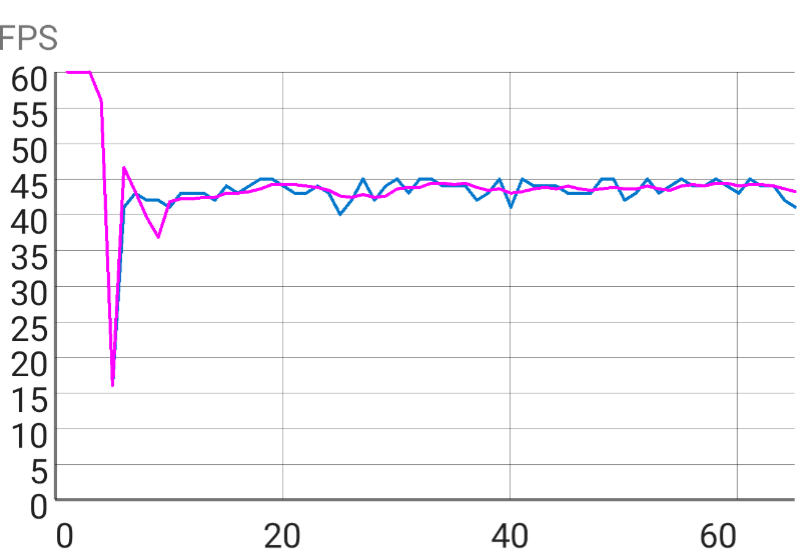
\includegraphics[width=\linewidth]{images/VRPerformance}
\caption{Quadros-por-segundo conforme o OVR Metrics Tool executado durante o funcionamento da aplicação }
\label{fig:VRPerformanceChart}
\end{figure}

A aplicação apresentou taxa média de 43.96 \textit{fps} (\textit{frames-per-second}, quadros-por-segundo), com mínima de 16 \textit{fps} e máxima de 60 \textit{fps}. Conforme representado pela figura \ref{fig:VRPerformanceChart}, a aplicação não mantém estáveis 60 \textit{fps} e isto se deve principalmente ao \textit{garbage collector} e à possíveis otimizações em código de GPU.

Durante a execução da aplicação, percebeu-se que quando a movimentação do cursor é mais veloz que a taxa de atualização, i.e., o \textit{update}, os pontos de ruído não são visualizados de maneira contínua, provocando o efeito visto na figura \ref{fig:filter02}, onde as partículas concentram-se em apenas alguns pontos amostrados pelo \textit{framerate} da aplicação \textit{Unity}, gerando regiões ruidosas espaçadas entre si.

Na figura \ref{fig:filter01} e \ref{fig:filter02} verifica-se que a linha azul forma-se de maneira estável ao longo do caminho percorrido pelo cursor, enquanto os pontos vermelhos se espalham ao redor desse caminho, indicando que a amplitude máxima de instabilidade é cerca de duas vezes maior que o tamanho do cursor, ou seja, facilmente perceptível pelo usuário e que impossibilitaria a realização de movimentos precisos e estáveis, em outras palavras, a exatidão e responsividade esperadas do controlador não são satisfatórias.

\begin{figure}[h!]
\centering
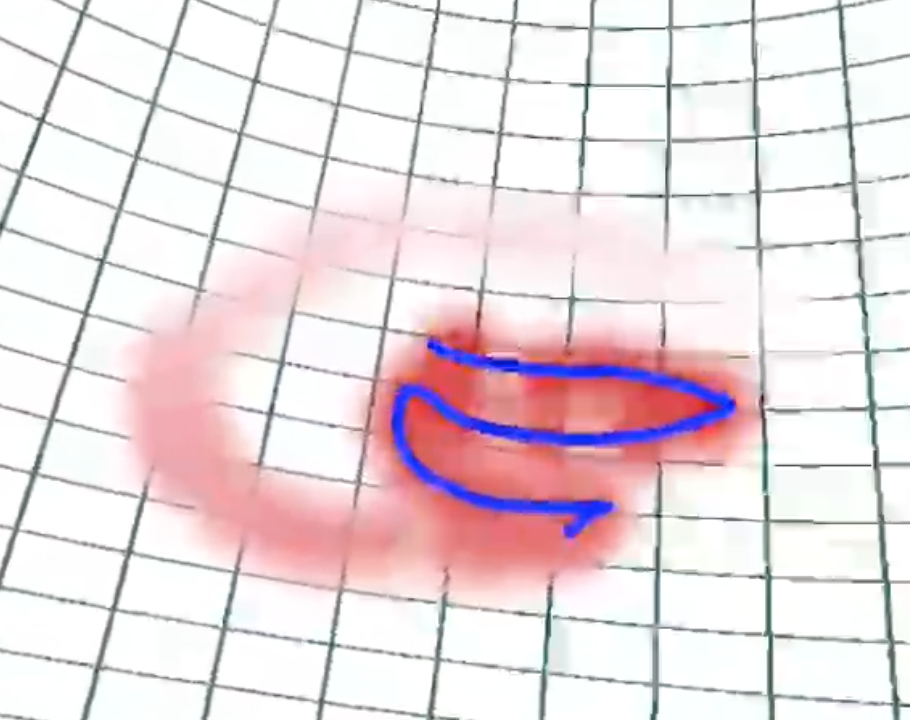
\includegraphics[width=\linewidth]{images/image_01.png}
\caption{Filtragem do cursor de VR. Amostras ruidosas em vermelho e valor filtrado em azul.}
\label{fig:filter01}
\end{figure}

\begin{figure}[h!]
\centering
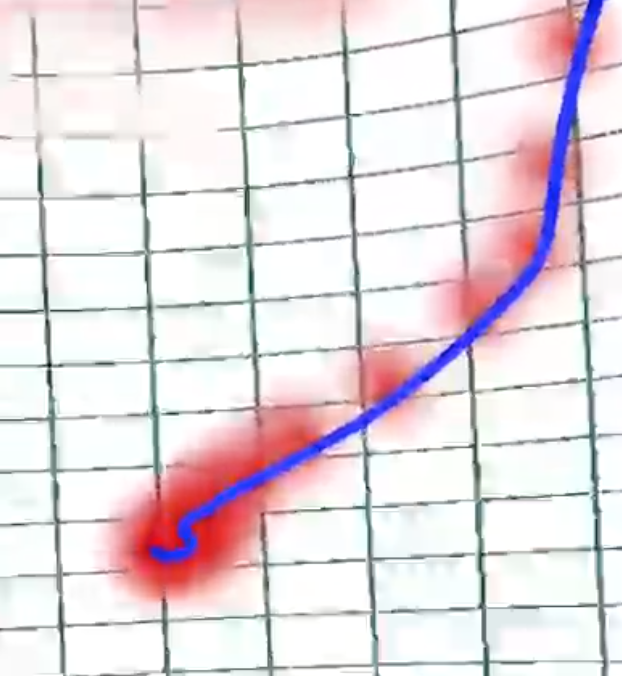
\includegraphics[width=\linewidth]{images/image_02.png}
\caption{Filtragem do cursor de VR. Amostras ruidosas em vermelho e valor filtrado em azul.}
\label{fig:filter02}
\end{figure}

\FloatBarrier % this prevents problems with misplaced pictures

A figura \ref{fig:chart_noise} mostra o gráfico da velocidade do curso ao longo da execução da aplicação. Ao comparar com o gráfico da figura \ref{fig:chart_filtered} gerado na mesma execução mas com o cursor filtrado, observamos que este último possui uma curva mais suave, indicando que o filtro de Kalman foi capaz de filtrar o ruído e assim suavizando o posicionamento capturado pelo controle.

\begin{figure}[h!]
\centering
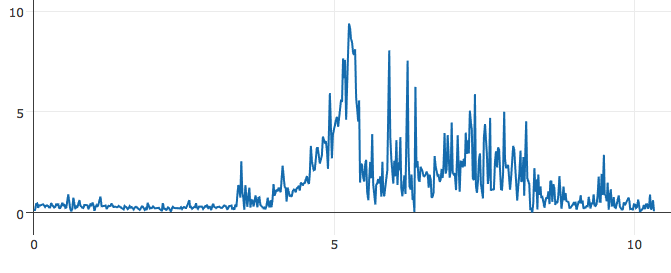
\includegraphics[width=\linewidth]{images/chart_noise.png}
\caption{Gráfico da velocidade do curso ao longo de uma execução da aplicação}
\label{fig:chart_noise}
\end{figure}

\begin{figure}[h!]
\centering
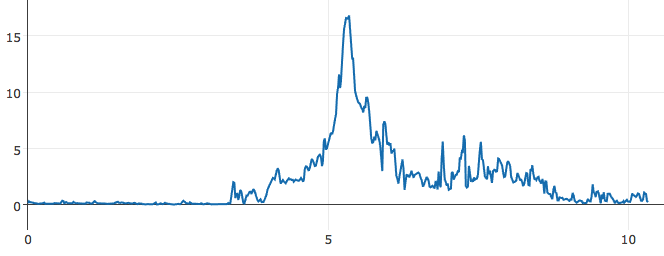
\includegraphics[width=\linewidth]{images/chart_filtered.png}
\caption{Gráfico da velocidade filtrada do curso ao longo de uma execução da aplicação}
\label{fig:chart_filtered}
\end{figure}
\FloatBarrier
%-------------------------------------------------------------------------------------------------
\section{Conclusão} \label{sec:conclusion}

Apresentou-se neste artigo a implementação do filtro de Kalman para estabilização do controle de realidade virtual da Oculus, o \textit{Gear VR Controller}. Concomitantemente, descreveu-se a visualização das entradas ruidosas fornecidas pelo controle e o efeito resultante após a aplicação do filtro. Apresentou-se também a implementação do jogo \textit{VRSnake} criado segundo a arquitetura de renderização baseada em \textit{shaders}.

Através dos resultados obtidos, verificou-se que a solução desenvolvida em \textit{Unity} para a aplicação do filtro foi efetivamente capaz de filtrar as posições ruidosas geradas pelo controlador e garantir um nível de controle mais estável em aplicações de realidade virtual. Da mesma maneira, o objetivo inicial de aliviar o trabalho de renderização atribuído à CPU foi alcançado por meio da distribuição de passos usualmente restritos à camada de aplicação para demais camadas da \textit{pipeline} gráfica.

% Trabalhos Futuros
Em trabalhos futuros, três passos são percebidos como cruciais. Em primeiro lugar, migrar inteiramente os processos da camada lógica para a camada de visualização, na unidade gráfica de processamento, com o propósito de permitir o controle e exibição de um número representativamente maior de serpentes. Em segundo lugar, aplicar aprendizagem de máquina nesta camada, objetivando-se um comportamento de busca e desvio de obstáculos (como outras serpentes e seu próprio corpo) mais inteligente, por conseguinte, desafiador. Por último, otimizar a performance objetivando maior fluidez.

\bibliographystyle{abbrv}
\bibliography{vrsnake_sbgames19}


% that's all folks
\end{document}


